\documentclass[final,dvipdfmx]{beamer}
\title{A proposal for semantic segmentation model for evaluating Gleason patterns of prostate cancer and integrated diagnostic system using Raspberry Pi}
\author{Ken Enda}
\institute{Department of Cancer Pathology Faculty of Medicine, HOKKAIDO UNIVERSITY }

% \usetheme{Rochester}
\usetheme{Berlin}

\usepackage{bxdpx-beamer}
\usepackage{pxjahyper}
\usepackage[orientation=portrait,size=a0,scale=1.4,debug]{beamerposter}
\usepackage[japanese]{babel}
\usepackage[font=small]{caption}
\usepackage[font=footnotesize]{subcaption}
\setbeamertemplate{navigation symbols}{}

% caption
\addto\captionsjapanese{\renewcommand{\figurename}{Fig}}
\addto\captionsjapanese{\renewcommand{\tablename}{Table}}
\setbeamertemplate{caption}[numbered]

% bin
\renewcommand{\kanjifamilydefault}{\gtdefault}
\setbeamercolor{bibliography item}{fg=black}
\setbeamercolor{bibliography entry author}{fg=black}
% \setbeamercolor{bibliography entry author}{fg=red}
% \setbeamercolor{bibliography entry title}{fg=blue}
% \setbeamercolor{bibliography entry location}{fg=green}
% \setbeamercolor{bibliography entry note}{fg=cyan}

% fig
\makeatletter
\def\@cite#1{\textsuperscript{[#1]}}
\makeatother

\begin{document}
\nocite{*}

\begin{columns}[T]
  \begin{minipage}[]{0.75\columnwidth}
    \vspace{5mm}
    \huge 前立腺癌のGleason pattern評価のためのSemantic segmentationモデルと、Raspberry Piを利用した統合された診断システムの提案
    \\[5mm]
    \large 遠田 建\cite{student} \hspace{5mm} 伊勢 昂生\cite{student} \hspace{5mm} 石田雄介\cite{teacher} \hspace{5mm} 田中 伸哉\cite{teacher}
    {\small
      \begin{thebibliography}{99}
        \beamertemplatetextbibitems
        \setlength{\itemsep}{-.5zw}
        \begin{minipage}[]{0.25\columnwidth}
          \bibitem{student} 北海道大学医学部医学科6年次
        \end{minipage}
        \begin{minipage}[]{0.40\columnwidth}
          \bibitem{teacher} 北海道大学大学院医学研究院腫瘍病理学教室
        \end{minipage}
      \end{thebibliography}
    }

  \end{minipage}

  \begin{minipage}[]{0.08\columnwidth}
    \begin{figure}\centering
      
\includegraphics[width=\columnwidth]{assets/logo_patho2.png}
    \end{figure}
  \end{minipage}

  \begin{minipage}[]{0.08\columnwidth}
    \begin{figure}\centering
      
\includegraphics[width=\columnwidth]{assets/logo_humed.png}
    \end{figure}
  \end{minipage}

  \begin{minipage}[]{0.08\columnwidth}
    \begin{figure}\centering
      
\includegraphics[width=\columnwidth]{assets/logo_hu.png}
    \end{figure}
  \end{minipage}
\end{columns}

\vspace{10mm}

\begin{columns}[T]
  \begin{column}{0.49\columnwidth}
    \begin{block}{\Large Introduction}
      \begin{flushleft}
         近年、Deep learning(DL)を用いた画像解析技術の発展は目覚ましいものがあり、病理組織画像を対象とした研究も大きな成果を挙げている。その一方で、臨床診断の現場において実際にその技術と成果物を使用する機会は極めて少ない。病理組織画像に対するDLによる推論結果を得るために、いくつかの段階を経る必要があるためである。まず、病理組織を撮影し、DLによってその画像を解析し、その結果を確認する。この工程には、画像ファイルを外部ストレージに持ち出したり、鏡検室と物理的には離れたDLシステムへ出歩くことも含まれるかもしれない。すぐれたDLSが存在しても、これらのような手間ゆえに臨床現場と直接結びにくくなっている。\par
\vspace{0.5zh}
 本研究ではRaspberry Piを用いて臨床診断の行われる顕微鏡とDLの動作環境をシームレスに結びつける仕組みを提案する。\par

      \end{flushleft}
    \end{block}

    \begin{block}{\Large Material and method}
      \begin{flushleft}
         我々はまず、前立腺の病理画像をGP(Gleason pattern)に応じて正常腺管、GP3、GP4、GP5のセマンティックセグメンテーション(Semantic segmentation、画像を意味に基づいてピクセル単位で区分する手法)を行うU-Net\cite{unet}モデルを作成した。U-NetモデルのエンコーダーはVGG16\cite{vgg}を使用し、さらに転移学習を行っている\cite{ternausnet}。デコーダーには逆畳込みではなくNearest samplingを用いた。\par

\vspace{0.5zh}

 モデルは当教室で診断された前立腺全摘出標本とFig\ref{fig:seg_color}のようなラベル付けによって訓練した。モデルの出力例をFig\ref{fig:dl_sample}に示す。\par

\vspace{-1zh}

\begin{figure}[htbp]\centering
  \begin{tabular}{c}
    \begin{subfigure}[t]{0.16\columnwidth}\centering
      
\includegraphics[width=0.7\columnwidth]{assets/gp_pin.png}
      \subcaption{正常腺管:黒}
    \end{subfigure}

    \begin{subfigure}[t]{0.16\columnwidth}\centering
      
\includegraphics[width=0.7\columnwidth]{assets/gp_3_2.png}
      \subcaption{GP3:青}
    \end{subfigure}

    \begin{subfigure}[t]{0.16\columnwidth}\centering
      
\includegraphics[width=0.7\columnwidth]{assets/gp_4.png}
      \subcaption{GP4:緑}
    \end{subfigure}

    \begin{subfigure}[t]{0.16\columnwidth}\centering
      
\includegraphics[width=0.7\columnwidth]{assets/gp_5_2.png}
      \subcaption{GP5:赤}
    \end{subfigure}

    \begin{subfigure}[t]{0.16\columnwidth}\centering
      
\includegraphics[width=0.7\columnwidth]{assets/gp_3_1.png}
      \subcaption{GP3+4}
    \end{subfigure}

    \begin{subfigure}[t]{0.16\columnwidth}\centering
      
\includegraphics[width=0.7\columnwidth]{assets/gp_5_1.png}
      \subcaption{GP4+5}
    \end{subfigure}
  \end{tabular}
  \label{fig:example}
  \caption{セグメンテーションによる色分け例}
  \label{fig:seg_color}
\end{figure}

\begin{figure}[htbp]\centering
  \begin{tabular}{c}
    \begin{subfigure}[t]{0.33\columnwidth}\centering
      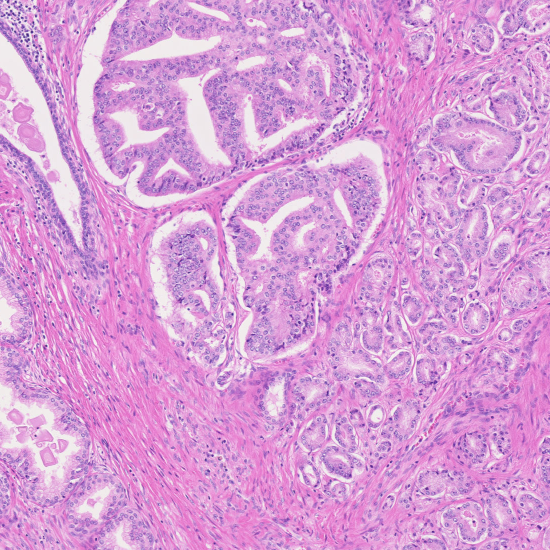
\includegraphics[width=0.9\columnwidth]{assets/ex_org.png}
      \subcaption{入力画像}
    \end{subfigure}

    \begin{subfigure}[t]{0.33\columnwidth}\centering
      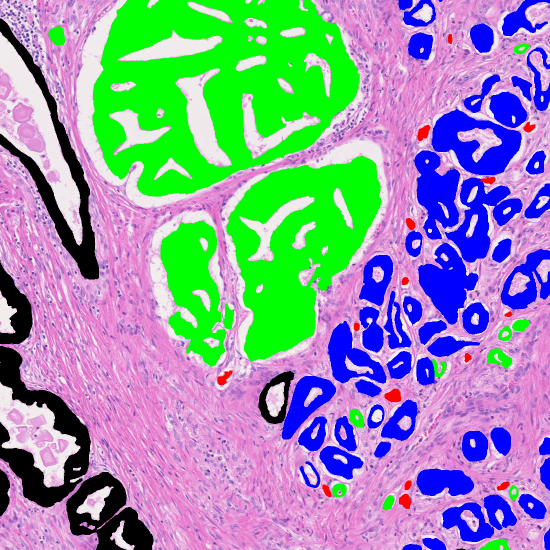
\includegraphics[width=0.9\columnwidth]{assets/ex_gt.png}
      \subcaption{ラベル画像}
    \end{subfigure}

    \begin{subfigure}[t]{0.33\columnwidth}\centering
      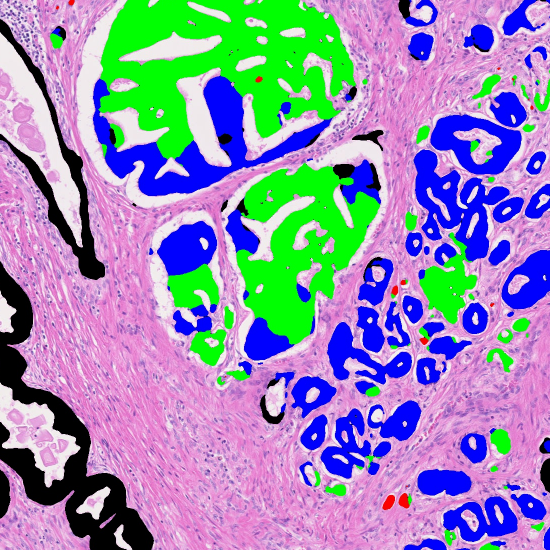
\includegraphics[width=0.9\columnwidth]{assets/ex_pr.png}
      \subcaption{出力画像}
    \end{subfigure}
  \end{tabular}
  \label{fig:example}
  \caption{U-Netモデルによる出力例}
  \label{fig:dl_sample}
\end{figure}

 作成したU-NetモデルのIoUはJaccard index(\ref{eq:iou})によって算出し、訓練画像に対して0.765、学習に含めなかったテスト画像に対して0.737であった。

\begin{equation}
\label{eq:iou}
  Jaccard\,index = \frac{|PR \cap GT|}{|PR \cup GT|}
\end{equation}

\vspace{0.5zh}

 さらに、USBカメラから入力された画像をHTTPによってネットワーク経由で送信するクライアントアプリケーションと、受信した画像をDLによって解析しその結果を配信するサーバーアプリケーションを作成した(Fig\ref{fig:arch})。前者は顕微鏡カメラとUSB接続したRaspberry Pi 4 Model Bに、後者はDLの動作するコンピュータにそれぞれ導入した。\par

\vspace{1zh}

\begin{figure}\centering
  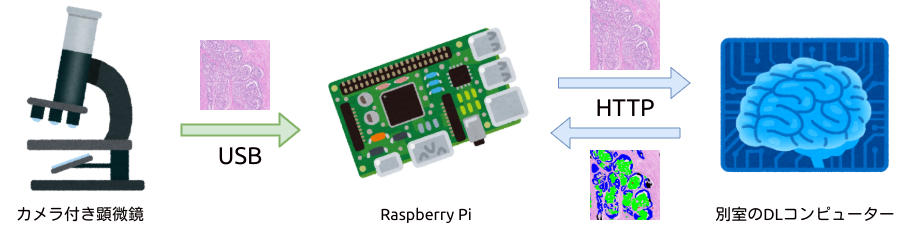
\includegraphics[width=\columnwidth]{assets/arch.png}
  \caption{クライアント・サーバーアプリケーション構成図}
  \label{fig:arch}
\end{figure}

\vspace{1zh}

 

      \end{flushleft}
    \end{block}

  \end{column}

  \begin{column}{0.49\columnwidth}

    \begin{block}{\Large Result}
      \begin{flushleft}
      mate  画像
画像
画像



      \end{flushleft}
    \end{block}

    \begin{block}{\Large References}
      \begin{figure}
        \begin{flushleft}
          \beamertemplatetextbibitems
          \bibliographystyle{junsrt}
          \bibliography{refs}
        \end{flushleft}
      \end{figure}
    \end{block}

  \end{column}

\end{columns}

\end{document}
